%% ####################### README  #######################
%% This document has been created with Vim. It uses 
%% the following non-standard packages:
%% - biblatex (with customized authoryear-aec style
%% 
%% This document is release
%% Copyright (C) 2010  Francesco de Virgilio <fradeve11@gmail.com>
%%
%% You can redistribute this document and/or
%% modify it under the terms of the GNU General Public License
%% as published by the Free Software Foundation; either version 2
%% of the License, or (at your option) any later version.

%% This program is distributed in the hope that it will be useful,
%% but WITHOUT ANY WARRANTY; without even the implied warranty of
%% MERCHANTABILITY or FITNESS FOR A PARTICULAR PURPOSE.  See the
%% GNU General Public License for more details.

%% You should have received a copy of the GNU General Public License
%% along with this program; if not, write to the Free Software
%% Foundation, Inc., 51 Franklin Street, Fifth Floor, Boston, MA  02110-1301, USA.
%% ####################### README  ####################### 

%%% TODO
%%% - correggere citazioni bibliografia
%%%


%% tipo di documento
\documentclass{paper}

%% [lingua] definizione della/e lingua/e; la lingua di default del documento è sempre l'*ultima*
\usepackage[english,french,italian]{babel}
\usepackage[utf8]{inputenc}
\usepackage[T1]{fontenc}

%% [biblatex] introduzione pacchetti utili per BibLaTeX
\usepackage[babel]{csquotes}
\usepackage[bibstyle=authoryear-aec,firstinits=true,citestyle=authoryear-comp,babel=hyphen,natbib=true,hyperref]{biblatex}

%% [biblatex] indico il nome del file .bib della bibliografia
\bibliography{bibliografia-grass-biblatex}

%% [geometria] stabilisco i margini
\usepackage[letterpaper]{geometry}
\geometry{verbose,lmargin=3cm,rmargin=3cm}

%% [immagini]
\usepackage{float}
\usepackage{graphicx}

%% [links] opzioni hyperref
\usepackage[unicode=true,bookmarks=true,bookmarksnumbered=false,bookmarksopen=false,breaklinks=true,pdfborder={0 0 1},backref=false,colorlinks=false]{hyperref}
\hypersetup{pdfauthor={Francesco de Virgilio}}

\begin{document}

%%%%%%%%%%%%%%%%%%%%%%%%%%%%%%%%%%%%%%%%%%%%%%%%%%%%%%%%%%%%%%%%%%%%%%%%%%%%%%%%
% CORREZIONI DI STILE %
%%%%%%%%%%%%%%%%%%%%%%%%%%%%%%%%%%%%%%%%%%%%%%%%%%%%%%%%%%%%%%%%%%%%%%%%%%%%%%%%

%% aggiunge una virgola tra Autore e anno nello stile citazione authoryear
\renewcommand{\nameyeardelim}{, }

%% sostituisce le parentesi tonde dell'anno di pubblicazione con "niente"
\renewcommand{\bibleftparen}{}
\renewcommand{\bibrightparen}{}

%% separa gli elementi della citazione con una virgola anzichè i punti
\renewcommand*{\newunitpunct}{\addcomma\space}

%% rende corsivo il titolo dell'articolo
\DeclareFieldFormat[article]{title}{\mkbibemph{#1}}

%% aggiunge "«»" al nome del giornale di pubblicazione, e fa seguire da una virgola
\DeclareFieldFormat{journaltitle}{\guillemotleft{#1}\guillemotright ,}
\DeclareFieldFormat{pages}{{#1}}

%%%%%%%%%%%%%%%%%%%%%%%%%%%%%%%%%%%%%%%%%%%%%%%%%%%%%%%%%%%%%%%%%%%%%%%%%%%%%%%%
% FINE CORREZIONI DI STILE %
%%%%%%%%%%%%%%%%%%%%%%%%%%%%%%%%%%%%%%%%%%%%%%%%%%%%%%%%%%%%%%%%%%%%%%%%%%%%%%%%

\title{L'impiego di \emph{mobile GIS} open source in Archeologia}

\subtitle{I progetti Tellus e Total Open Station}

\author{Francesco de Virgilio\thanks{\protect\href{mailto:fradeve11@gmail.com}{fradeve11@gmail.com}, Corso di Laurea Triennale in Scienza e Tecnologia per la Diagnostica e Conservazione dei Beni Culturali}}

\institution{Universit\`{a} degli Studi di Bari - Dipartimento Geomineralogico}

\date{Gennaio 2010}
\maketitle

\begin{abstract}
Questo scritto mostra come il software incluso nel progetto open source
Tellus sia un valido strumento per creare una rete di comunicazione
in tempo reale tra il cantiere di scavo e l'ufficio, permettendo agli
archeologi di scambiare informazioni geografiche, grazie all'utilizzo
di un GIS portatile e completo. Tellus può essere eseguito anche su
dispositivi portatili economici e aperti, ed in generale fornisce
una serie di funzioni utili al lavoro sul campo (possibilità di lavorare
senza collegamento alla rete, motore di sincronizzazione, compatibilità
con differenti tipi di database, \ldots). Tellus, in coppia con software
open source installabili su server come PostGIS e MapServer, offre
la possibilità di generare WMS quasi in tempo reale, accessibili da
tutto il mondo attraverso Internet sia per la visualizzazione che
per la modifica dei dati tramite query sul database. Il software libero
Total Open Station, creato secondo processi di sviluppo comunitari,
installato su dispositivi con sistema operativo GNU/Linux, offre la
possibilità di trasferire i dati direttamente dalla stazione totale
all'ufficio, evitando l'uso di computer e di software proprietario.\\


This paper shows that the software included in the open source Tellus
Project is a valid tool to create a network of real-time communication
among field and office, enabling archaeologists to share geographic
informations using a full featured portable GIS. Tellus could be executed
also on cheap open-hardware mobile devices, and in general provides
a series of useful features (possibility to work in disconnected mode,
synchronization engine, works with any type of database, \ldots).
Tellus software suite in combination with open source server-side
software like PostGIS and MapServer offers the possibility to generate
near-real-time WMS, accessible through the Internet from all the world
both for view and database query. The community-driven Total Open
Station free software on GNU/Linux powered devices offers the possibility
to transfer data directly from total station to office, avoiding computers
and proprietary software.\end{abstract}

\begin{keywords}
Open Mobile~IS, gvSIG~mobile, PostGIS, MapServer, database, GIS,
stazione~totale, Total~Open~Station, sincronizzazione
\end{keywords}

\pagebreak{}

	L'obiettivo di questo scritto \`{e} riassumere alcune delle esperienze
	registrate negli ultimi anni a proposito della transizione dei sistemi
	GIS dal laboratorio all'area di scavo su dispositivi portatili, che
	ha portato ad un evidente snellimento dei tempi di raccolta dei dati.
	In questa breve introduzione alla sincronizzazione dei dati tra cantiere
	e laboratorio si tralasceranno alcuni aspetti tecnici del software,
	per porre l'accento sugli aspetti più utili ed interessanti nel contesto
	archeologico.\\


	\`{E} ampiamente dimostrato quanto l'archeologia stratigrafica sia legata
	ai metodi informatici per la documentazione, organizzazione, analisi
	e comunicazione dello scavo archeologico; \`{e} tuttavia interessante
	notare come alcuni passaggi tra queste fasi vadano notevolmente accorciandosi,
	grazie al contributo dell'ICT ed in particolar modo delle tecnologie
	open source, o comunque libere\footnote{Con la presente affermazione si intende
	aderenti ad una delle licenze riconosciute come ``libere'' dalla Free Software Foundation.}.

	Un numero sempre maggiore di archeologi decide di adottare software
	libero per organizzare il \emph{workflow archeologico}, e non \`{e} raro
	che il contributo sempre crescente di molte realt\`{a}, in questo grande
	{}``calderone'' del software libero per l'archeologia, porti allo
	sviluppo di applicazioni all'avanguardia nel settore rispetto ai competitor
	\emph{closed source}. Allo stato attuale, lo scenario --- non necessariamente
	futuristico --- della velocizzazione dei processi di rilievo/analisi
	a livello archeologico e dell'assenza di rivali commerciali simili
	sul mercato del software chiuso, vede il coinvolgimento di due attori:
	gvSIG Mobile e Open Mobile IS.\\


	Dall'unione di questi software \`{e} nato il progetto Tellus. L'idea di
	Tellus, che interseca le esperienze sul campo di Oxford Archaeology \footnote{\url{http://openarchaeology.net/}},
	\`{e} proprio quella di trasformare dei palmari economici in strumenti
	di documentazione/comunicazione in tempo reale, con l'obiettivo di
	trasmettere \emph{al volo} tutti i dati georiferiti dal cantiere di
	scavo all'ufficio. Questi risultati possono essere ottenuti soltanto
	progettando un'infrastruttura hardware e software adatta allo scopo,
	ed utilizzando programmi che supportino tutti i protocolli di comunicazione
	necessari al trasferimento e sincronizzazione dei dati. Entrambe queste
	caratteristiche sono facilmente ottenibili dal processo di sviluppo
	comunitario diffuso in ambito open source.


\section[gvSIG mobile, OpenMobile IS e Tellus]{gvSIG mobile, Open Mobile IS e Tellus\footnote{Ulteriori informazioni a proposito dell'integrazione dei due programmi
nel progetto Tellus possono essere reperite in un paper disponibile online ad opera degli autori di Tellus; si veda \cite{tellusarticle}.}}

	gvSIG\footnote{Sito ufficiale: \href{http://www.gvsig.gva.es}{http://www.gvsig.gva.es}} \`{e} un programma scritto in Java, multipiattaforma, per la gestione
	d'informazione geografica (\emph{GIS}) con precisione cartografica,
	distribuito con licenza GNU GPL. Permette di gestire dati vettoriali
	e raster e di connettersi a server cartografici con standard OGC\footnote{Una delle principali caratteristiche di gvSIG è l'implementazione
	di servizi OGC: WMS (\emph{Web Map Service}), WCS (\emph{Web Coverage
	Service}), WFS (\emph{Web Feature Service}).}. gvSIG \`{e} nato nel 2003, quando la Direzione Infrastrutture e Trasporti
	della Comunità Valenziana ha deciso di realizzare un proprio SIT.
	Il progetto \`{e} finanziato dall'Unione Europea, Fondo europeo di sviluppo
	regionale (FEDER).

	Recenti sviluppi del programma hanno portato alla creazione di una
	versione \emph{mobile}\footnote{Sito ufficiale: \href{http://www.gvsig.gva.es/eng/gvsig-mobile}{http://www.gvsig.gva.es/eng/gvsig-mobile};
	sito di riferimetno della versione non ufficiale per dispositivi GNU/Linux:
	\href{http://gvsigmobileonopenmoko.wordpress.com}{http://gvsigmobileonopenmoko.wordpress.com}.}, con funzioni ridotte rispetto a gvSIG, ottimizzata per essere eseguita
	su dispositivi dotati di sistema operativo GNU/Linux (fino ad ora
	lo smartphone FIC Openmoko --- in fig.~\ref{fig:Layer-gvSIG}, il
	tablet Nokia N800/N810 con sistema operativo Maemo --- Debian GNU/Linux,
	ed ovviamente qualsiasi dispositivo desktop, netbook compresi, con
	tale sistema operativo).\\


	Open Mobile IS (abbr. OpenMIS) \`{e} un progetto open source (licenza
	GNU GPL v. 2.1) che ha l'obiettivo di fornire un framework con tutti
	gli strumenti e le API per la creazione di applicazioni mobile. Open
	Mobile IS, in particolare, mette a disposizione:

\begin{description}

	\item [{database~integrato}] ottimizzato per funzionare con bassi consumi
	di CPU e RAM;

	\item [{motore~di~sincronizzazione}] che opera tra il database integrato
	del dispositivo e un database remoto (nel caso archeologico un database
	geografico PostGIS); il sistema di tracciamento delle modifiche tra
	i due database è basato su un \emph{numero di sincronizzazione incrementale};
	si evita in questo modo di tracciare le modifiche in base alla data,
	eliminando la necessit\`{a} che entrambi i dispositivi che ospitano i
	database abbiano orologi di sistema sincronizzati (caratteristica
	molto ultile sul cantiere di scavo).

\end{description}

	Dall'integrazione di OpenMIS in gvSIG mobile \`{e} nato il progetto Tellus\footnote{Sito ufficiale: \href{http://tellusproject.blogspot.com/}{http://tellusproject.blogspot.com/}}, che unisce le capacit\`{a} di sincronizzazione e risoluzione dei conflitti
	dei dati geografici del primo con le caratteristiche GIS del secondo.

\section{Applicabilità pratica}

	La flessibilit\`{a} del software libero ed in generale il generoso hardware
	dei dispositivi supportati da gvSIG mobile, precedentemente citati,
	sono di fondamentale importanza per l'impiego in campo archeologico,
	considerate:

	\begin{itemize}
		\item le dimensioni notevolmente ridotte rispetto ad un laptop o ad un computer
			desktop;
		\item il costo mediamente contenuto per l'hardware (a cui si aggiunge la
		  	gratuit\`{a} del software);
		\item la notevole autonomia energetica, incrementabile con batterie aggiuntive
			dal costo relativamente basso;
		\item l'alta connettivit\`{a} (in media tali dispositivi sono dotati di wifi,
			bluetooth, e supportano connessioni dati GPRS; Openmoko e Nokia N810
			hanno un ricevitore GPS integrato);
		\item le porte di comunicazione standard (mini-USB).
	\end{itemize}
	
	Questi due ultimi punti rivestono un'importanza fondamentale nel lavoro
	sul campo, soprattutto perch\'{e} la connettività \`{e} il fulcro del nuovo
	modo di intendere la documentazione dello scavo archeologico.\\

	L'infrastruttura nel suo complesso, raffigurata schematicamente in
	fig.~\ref{fig:schema_tellus} \`{e} costituita da una serie di client
	(ovvero tutti i dispositivi utilizzati sul campo: palmari, tablet,
	notebook e netbook, raffigurati sulla sinistra) sui quali \`{e} stato
	installato Tellus, e da un server localizzato nel laboratorio, equipaggiato
	con sistema operativo GNU/Linux, su cui sono installati MapServer
	e un database PostGIS (entrambi open source). A questi due fronti
	di scambio del dato archeologico se ne aggiunge un terzo, quello dei
	computer degli operatori in ufficio, che collegandosi al database
	PostGIS sul server possono visualizzare in tempo reale il flusso dei
	dati dal campo, e quindi lavorare ed elaborare la documentazione ``in
	diretta''. Tutti gli elementi di questa rete comunicano tra loro
	tramite una normale connessione ad internet.\\

	Prima dello scavo l'intera cartografia a disposizione, omogeneizzata
	in un formato compatibile con gvSIG (ad esempio SHAPEfile, ma gli
	sviluppatori hanno documentato anche l'utilizzo di WKT) e opportunamente
	divisa in layer, viene caricata sul server. Durante le quotidiane
	operazioni di documentazione, i fogli quadrettati, i fili a piombo
	e lo scalimetro vengono sostituiti dai più veloci ed efficienti palmari,
	netbook e stazione totale; la carta cede il passo ad un layer sul
	GIS nel palmo della mano dell'operatore. Il dispositivo palmare connesso
	ad internet scambia in tempo reale informazioni con il server, aggiornando
	simultaneamente i layer vettoriali e raster.

	Il rilievo viene effettuato:
	
	\begin{enumerate}
		\item con l'utilizzo della stazione totale;
		\item aggiungendo a mano direttamente sul layer del GIS mobile le informazioni.
	\end{enumerate}

	Nel primo caso, non sar\`{a} necessario arrivare nel laboratorio sul campo
	per inviare i dati direttamente dalla stazione totale all'ufficio:
	gli sforzi di Stefano Costa e Luca Bianconi hanno portato alla creazione
	di Total Open Station\footnote{\href{http://tops.berlios.de/}{http://tops.berlios.de/}},
	software (ben integrato con Openmoko) che permette di scaricare
	i dati direttamente dalla stazione sul palmare, dal quale potrebbero
	essere eventualmente inviati in ufficio via wifi o GPRS.

	Nel secondo caso, tutte le informazioni rilevate vengono sincronizzate
	con il server PostGIS via internet (quindi usando una connessione
	wifi o GPRS laddove possibile) e messe a disposizione dei ricercatori
	collegati al server PostGIS, teoricamente da qualsiasi punto del mondo.
	Se nel server \'{e} installato ed opportunamente configurato MapServer,
	\'{e} possibile impostarlo per aggiornare ad intervalli regolari la mappa
	raster partendo dal database, in maniera tale da poter offrire ai
	ricecatori connessi un WMS quasi in tempo reale. La configurazione
	di un eventuale interfaccia web per la visualizzazione del WMS o in
	generale di cartografia archeologica gode di una tradizione ormai
	consolidata in ambito open source (\cite{geoportali-archeologia} e \cite{webmapping-arch}),
	grazie all'utilizzo di software come p.mapper o OpenLayers.\\

	Il dispositivo portatile con Tellus non invia solo dati, ma contemporaneamente
	pu\`{o} riceverne, sia in forma vettoriale che raster, poichè gvSIG integra
	il supporto al WMS. Il trasferimento dei dati cartografici tra gvSIG
	mobile, OpenIMS e il server viene effettuato tramite il protocollo
	SOAP (una specifica XML). Il trasferimento effettivo dei file, come si vede in
	fig. \ref{fig:Schema-riassuntivo}, pu\`{o} avvenire in due maniere:
	
	\begin{itemize}
		\item Via HTTP, l'intero progetto cartografico viene trasferito in un unico
			archivio.
		\item Via Bittorrent, il palmare funge non solo da client, ma anche da server
			momentaneo per l'invio dei file cartografici ad altri palmari connessi
			alla rete, sincronizzando i file sull'intero parco macchine portatile;
			\'{e} raccomandata per la sincronizzazione di grandi quantità di dati,
			in quanto il torrent ha una migliore gestione della rete e di eventuali
			disconnessioni improvvise.
	\end{itemize}


\section{Conclusioni}

	Le applicazioni di un sistema di lettura e modifica di dati geografici
	in tempo reale sono molteplici e difficilmente riassumibili. L'applicabilità
	nel settore dei beni culturali, e particolarmente in quello archeologico,
	\'{e} limitata soltanto dal dover ottenere connettivit\`{a} sul cantiere di
	scavo, ma offre il vantaggio di unire i momenti del rilievo e dell'elaborazione
	dei dati, operazioni effettuate non necessariamente dagli stessi operatori,
	e non necessariamente nello stesso luogo fisico, accelerando il processo
	di ricerca e studio del patrimonio archeologico.

	Si apre al contempo la strada al concetto di \emph{open archaeology},
	avvicinando il patrimonio archeologico al cittadino, che se non pu\`{o}
	fisicamente recarsi sul luogo di scavo, potrebbe osservare l'evoluzione
	della ricerca archeologica quasi ``in diretta'' via internet;
	in maniera simile, si potrebbe filtrare l'accesso ai soli addetti
	ai lavori, o distribuire l'analisi su più punti diversi del territorio,
	o in più centri di ricerca nel mondo.

	La piena aderenza agli standard \emph{de facto} internazionali dal
	punto di vista informatico e l'adozione di software open source realizzato
	in maniera collaborativa, garantiscono la continuit\`{a} del processo
	di conoscenza, che in questo frangente diventa il filo conduttore
	tra Archeologia e Tecnologia.

%% stampa la bibliografia
%\addcontentsline{toc}{chapter}{\bibname}
\section*{Bibliografia}
\textsc{Chaumet A.} 2008, \emph{ Webmapping, arch{\'{e}}ologie et g{\'{e}}oportail}, «Archeologia e Calcolatori», 19, 79-86.\\

\noindent \textsc{Djindjian, F.} 2008, \emph{Webmapping in the historical and archaeological sciences. An introduction}, «Archeologia e Calcolatori», 19, 9-16.\\

\noindent \textsc{Gomez M., Delrieu P., Dom\'{i}nguez J.L.} 2009, \emph{The Tellus project}, (\url{https://svn.prodevelop.es/public/labs/gvsigmobileonopenmoko/webresources/media/tellus_article_5th_gvsig_conference.pdf}).

\pagebreak

	\begin{center}
	  \begin{figure}
	    \begin{center}
	      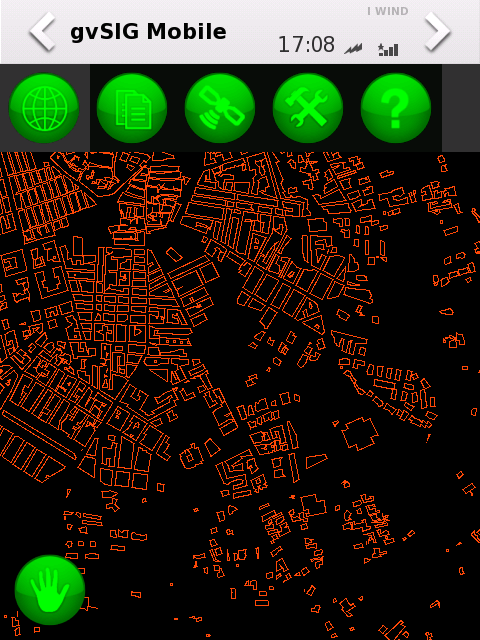
\includegraphics[scale=0.3]{img/screenshotGV.png}
	    \end{center}
	    \caption{\small{Layer vettoriale di edificato urbano
	    all'interno di gvSIG mobile su dispositivo Openmoko (\emph{Francesco de Virgilio}).}}
	    \label{fig:Layer-gvSIG}
	  \end{figure}
	\end{center}

	\begin{center}
	  \begin{figure}
	   \begin{center}
	    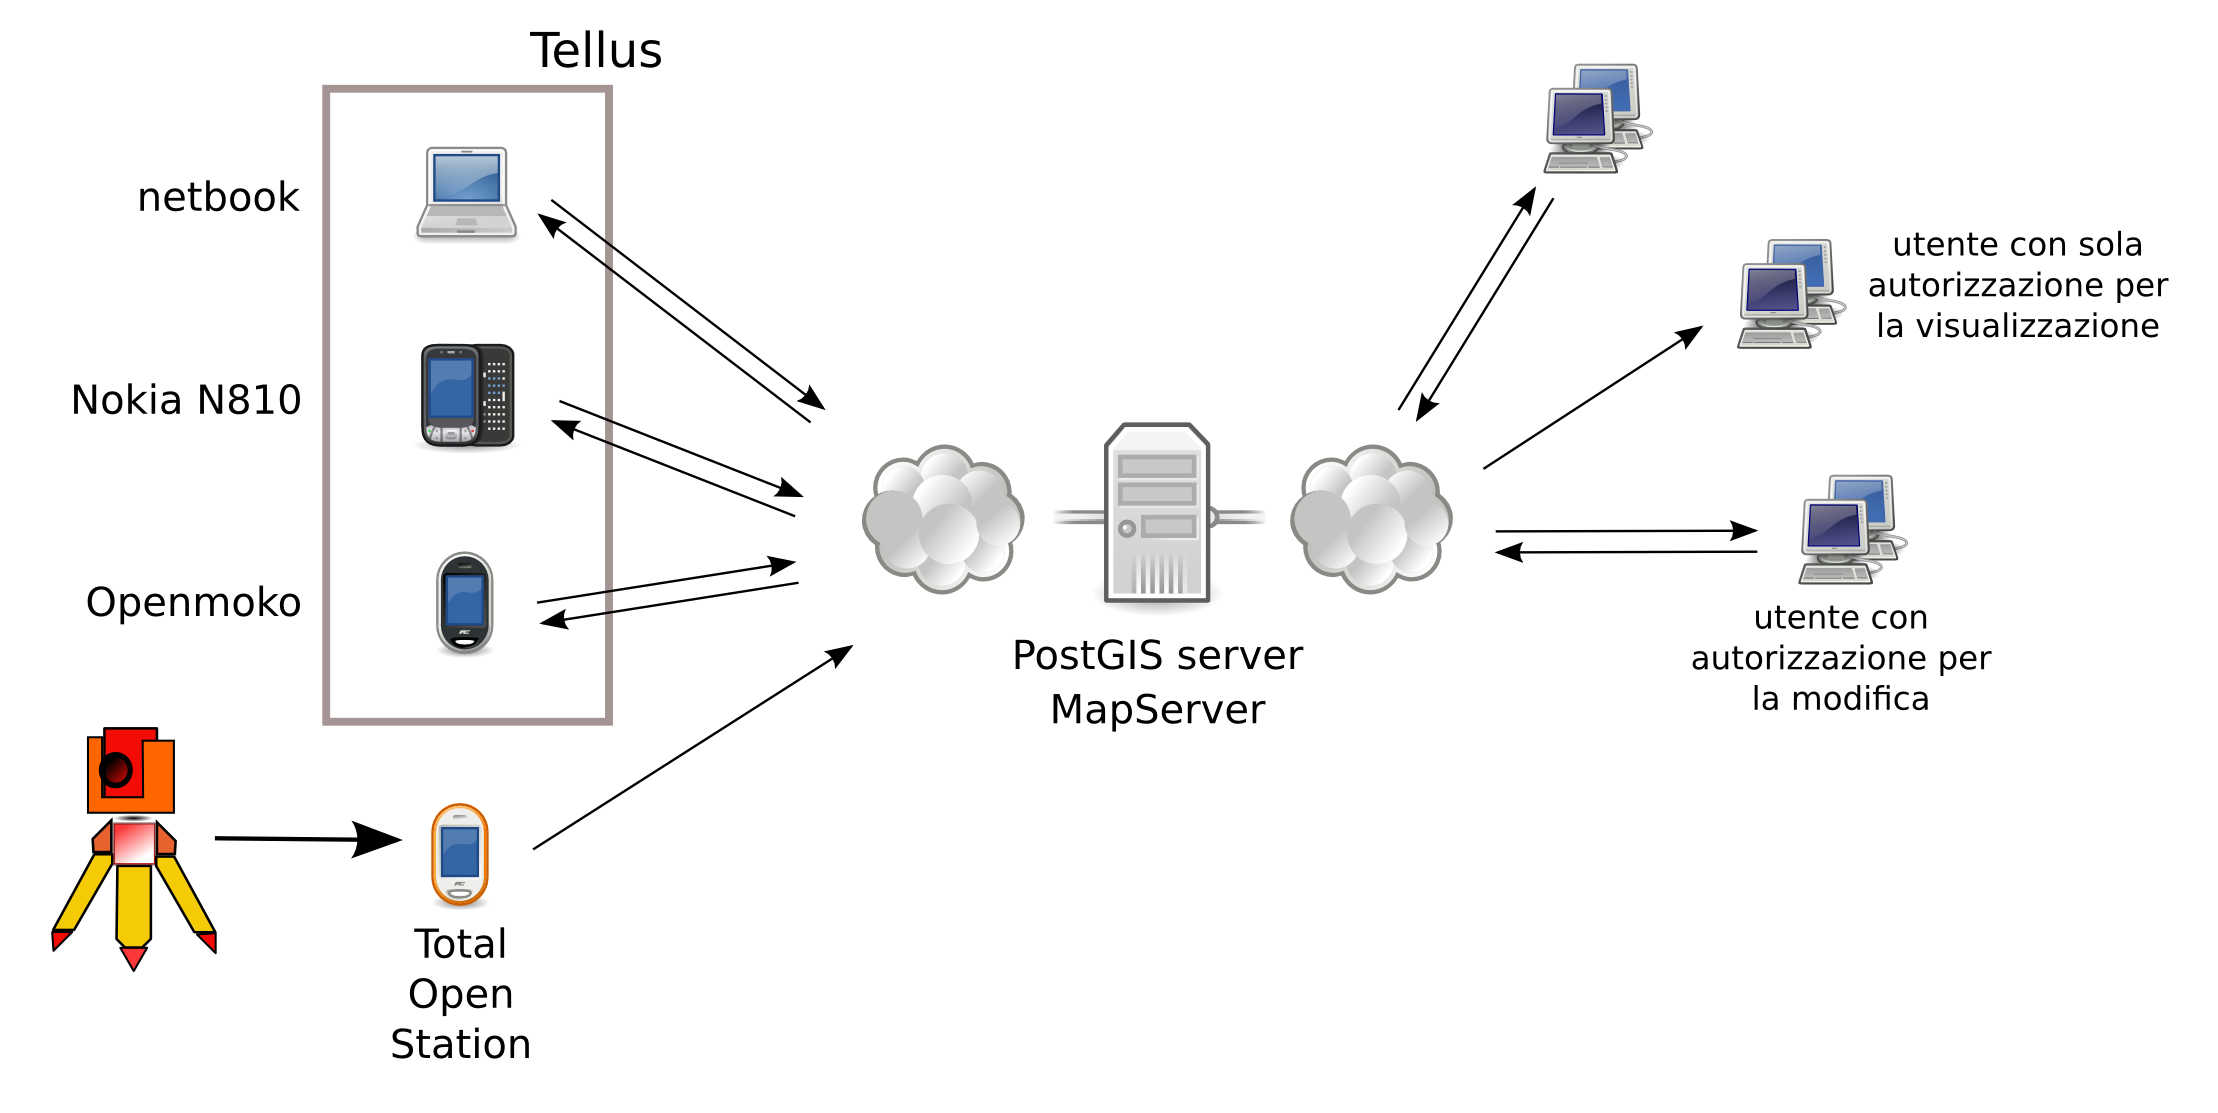
\includegraphics[scale=0.6]{img/schematellus.png}
	   \end{center}
	  \caption{\small{Raffigurazione schematica di un'infrastruttura
	 		di GIS mobile atta all'impiego in ambito archeologico (\emph{Francesco de Virgilio}).}}
	  \label{fig:schema_tellus}
	 \end{figure}
	\end{center}

	\begin{center}
	  \begin{figure}
	    \begin{center}
	      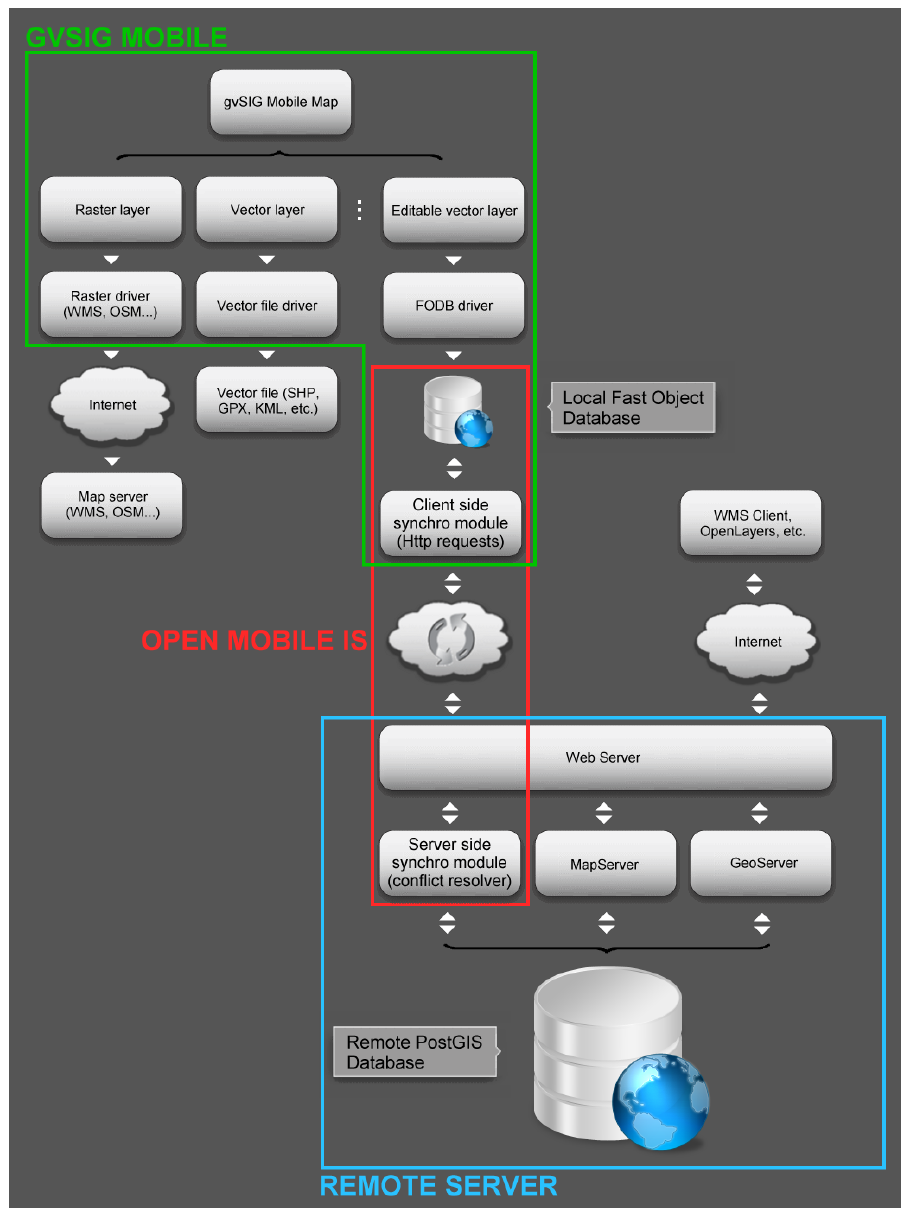
\includegraphics[scale=0.5]{img/generalscheme.png}
	    \end{center}
	    \caption{{\small Schema riassuntivo del funzionamento
			di OpenMIS, come struttura di collegamento tra gvSIG mobile e un server
			PostGIS (\emph{Juan~Lucas~Dom\'{i}nguez~Rubio}).}}
	    \label{fig:Schema-riassuntivo}
	  \end{figure}
	\end{center}

\end{document}
